% !TEX root = report.tex
\chapter*{Extended Abstract}

\begin{center}
	\begingroup
	\renewcommand*{\arraystretch}{1}
	\rowcolors{2}{white}{white}
	{\makeatletter	
		\begin{tabular}{p{3.2cm}p{9.6cm}}
			Thema: & \thema \\
			& \\
			Teammitglieder: & \verfasserA, \verfasserB, 
			\verfasserC, \verfasserD\\
			& \\
			Betreuer: & \hoschschule \newline \institut \newline \prueferA, \prueferB \\
			& \\
		\end{tabular}
		
		\makeatother}
	\endgroup
\end{center}

\bigskip

\noindent
Unser Projekt behandelt das r"aumliche Detektieren eines Modellhubschraubers. Die Detektion soll unter Laborbedingungen, das hei"st, der Helikopter befindet sich vor einer wei"sen Wand, stattfinden. Mittels der Detektion soll auf einem Bild angezeigt werden, wo sich der Mittelpunkt des Helikopters befindet. Auch die Tiefe (Entfernung zur Kamera) des Helikopters soll ermittelt werden. F"ur diese Detektion sollen zwei oder mehr Kameras verwendet werden. Bei diesen handelt es sich um HIERKAMERAEINF"UGEN, die mit dem Computer "uber ein FireWire-Kabel verbunden sind.\newline

\begin{figure}[H]
	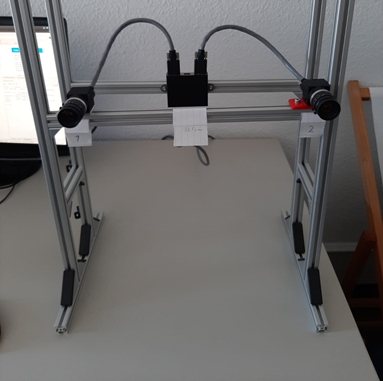
\includegraphics[scale=1.0]{bilder/camerasystem}
	\caption[Kamera-System]{Kamera-System}
\end{figure}

\noindent Das Projekt wurde erfolgreich umgesetzt.
Mittels zwei Kameras, die auf einer geraden Linie angebracht sind, kann der Mittelpunkt des Helikopters und dessen Abstand zur Kamera ermittelt werden.\newline
Unser Programm kalibriert als erstes die Kameras einzeln und anschlie"send zu einander. Das Kalibrieren erfolgt "uber ein Schachbrett-Muster. Sind die Kameras zueinander kalibriert, kann mittels eines Feature-Detektors eine Punktewolke des Helikopters generiert und der Mittelpunkt berechnet werden.

\begin{figure}%
	\centering
	\subfloat[Kamera-Kalibrierung]{{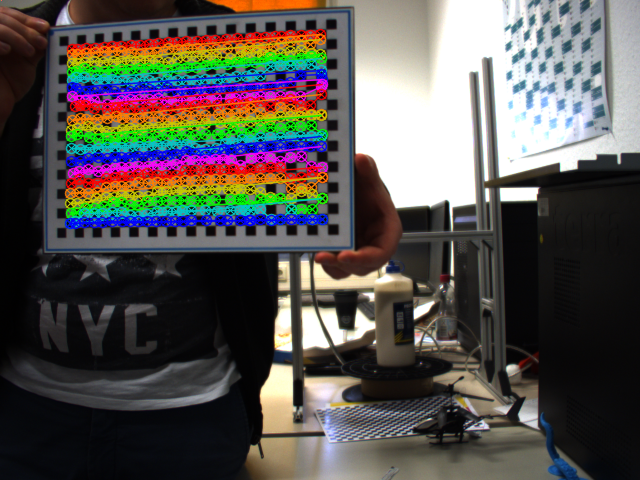
\includegraphics[width=6cm]{bilder/calibration} }}%
	\qquad
	\subfloat[Helikopter-Punktewolke]{{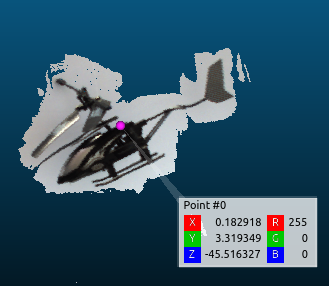
\includegraphics[width=6cm]{bilder/helicloud} }}%
	\caption{Kamera-Kalibrierung und Punktewolke}%
	\label{fig:example}%
\end{figure}
\noindent Eine m"ogliche Erweiterung des Projekts w"are das Kalibrieren von zwei Stereo-Systemen zu einander, um eine noch h"ohere Genauigkeit zu erlangen. Dies wurde versucht umzusetzen, ist allerdings gescheitert.

